\documentclass[a4paper, 11pt, final, garamond]{book}
\usepackage{cours-preambule}

\raggedbottom

\makeatletter
\renewcommand{\@chapapp}{Travaux pratiques -- TP}
\makeatother

\let\SavedIndent\indent
\protected\def\indent{%
  \begingroup
    \parindent=\the\parindent
    \SavedIndent
  \endgroup
}
\setlength{\parindent}{0pt}

\begin{document}
\setcounter{chapter}{11}

\chapter{Correction du TP}
\section{Objectifs}

\begin{itemize}
    \item Mise en place expérimentale d'un circuit RLC série. 
    \item Utiliser correctement des dispositifs de mesure de tension. 
    \item Vérifier les caractéristiques de la résonance en intensité d'un
        circuit RLC série. 
\end{itemize}

\section{Analyser}

\begin{enumerate}[label=\sqenumi]
    \item Pour vérifier la résonance en intensité, on doit envoyer un signal
        sinusoïdal dans le circuit et en observer l'intensité. On peut pour cela
        utiliser un générateur basses fréquences (un GBF), et observer à
        l'oscilloscope la tension aux bornes de $R$~: en effet, un oscilloscope
        ne mesure pas d'intensité mais que des tensions, cependant $u_R = Ri$
        donc visualiser $u_R$ revient à visualiser $i$ à un facteur près. Si on
        observe aux bornes de $u_L$, on observerait la dérivée de l'intensité,
        et aux bornes de $u_C$ son intégrale. Ainsi~:
        \begin{enumerate}
            \item On câble un circuit RLC série, avec $R$ en fin de circuit pour
                que sa masse soit confondue avec celle du générateur~;
            \item On relie la voie 1 de l'oscilloscope aux bornes du
                générateur~:
            \item On relie la voie 2 l'oscilloscope aux bornes de la
                résistance~;
            \item On observe les deux signaux sur l'oscilloscope, en réglant
                comme il se doit les trois éléments pour une bonne visualiation
                de signal (trigger, calibre vertical, calibre horizontal)~;
            \item En faisant varier la fréquence d'entrée sur le GBF, le signal
                de sortie varie en amplitude et en phase~: on relève donc pour
                différentes fréquences d'excitation l'amplitude du signal de
                sortie ainsi que son décalage temporel/sa phase par rapport à
                l'entrée~;
            \item On trace l'évolution de l'amplitude et de la phase en fonction
                de la fréquence~: dans le cadre de la résonance en intensité, on
                a toujours résonance à $\w_r = \w_0$, et les signaux sont en
                phase à la résonance. En deçà et au-delà de $\w_0$, l'amplitude
                décroît jusqu'à 0.
        \end{enumerate}

    \item On sait que $\w_0 = 1/\sqrt{LC} = 2\pi f_0$. Étant donné qu'on veut
        $f_0 = \SI{1}{kHz}$ et que $L = \SI{0.1}{H}$, on isole $C$ de
        l'équation~:
        \begin{gather*}
            2\pi f_0 = \frac{1}{\sqrt{LC}}
            \Leftrightarrow
            \sqrt{LC} = \frac{1}{2\pi f_0}
            \Leftrightarrow
            LC = \frac{1}{(2\pi f_0)^2}\\
            \boxed{
                C = \frac{1}{L(2\pi f_0)^2}
            }
            \qavec
            \left\{
                \begin{array}{rcl}
                    f_0 & = & \SI{1}{kHz} = \SI{1e3}{Hz}\\
                    L & = & \SI{0.1}{H}
                \end{array}
            \right.\\
            \mathrm{A.N.~:}\quad
            \boxed{
                C = \SI{2.53e-7}{F} = \SI{0.253}{\micro F}}
        \end{gather*}
        $R$ n'intervient pas dans le choix de la fréquence de résonance~; elle
        intervient cependant dans l'expression du facteur de qualité $Q$. On a
        \begin{gather*}
            Q = \frac{1}{R} \sqrt{\frac{L}{C}}
            \Leftrightarrow
            \boxed{R = \frac{1}{Q} \sqrt{\frac{L}{C}}}
        \end{gather*}
        On choisit un $Q$ un peu grand avec une valeur de résistance
        réalisable~: $Q = 3$ implique d'utiliser une résistance de
        \fbox{$\SI{210}{\Omega}$}.
    \item On réalise le montage suivant~:

        \begin{minipage}{0.40\linewidth}
            \begin{center}
                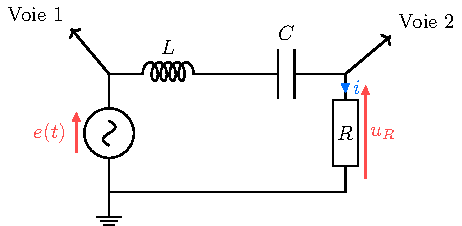
\includegraphics[width=\linewidth]{rlc_r-right}
            \end{center}
        \end{minipage}
        \hfill
        \begin{minipage}{0.55\linewidth}
            En effet, lorsque deux voies sont branchées sur l'oscilloscope, elles
            partagent la même masse, c'est-à-dire la même référence de potentiel (la
            masse a un potentiel nul~: c'est depuis ce point qu'on mesure les
            tensions par différences de potentiels).
        \end{minipage}
        \begin{minipage}{0.55\linewidth}
            Ainsi, si la résistance n'est pas à la fin du circuit, on ferait le
            circuit ci-contre~; dans ce cas, comme les masses sont
            automatiquement reliées entre elles \textit{via} l'oscilloscope, on
            créerait un court-circuit aux bornes de $C$ (on se retrouve avec un
            circuit $RL$).
        \end{minipage}
        \hfill
        \begin{minipage}{0.40\linewidth}
            \vspace{-10pt}
            \begin{center}
                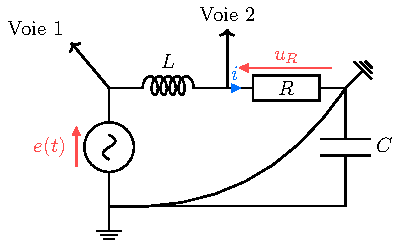
\includegraphics[width=.8\linewidth]{rlc_r-wrong}
            \end{center}
        \end{minipage}

        On règle donc $R$ sur $\SI{210}{\Omega}$, $C$ sur \SI{0.253}{\micro F}
        et on utilise $L$ d'inductance \SI{0.1}{H}. Pour le générateur, on
        vérifie en premier lieu la fréquence de résonance en se plaçant à
        \SI{1}{kHz} en mettant la fiche sur l'\texttt{OUTPUT} de la ligne du
        haut, bouton \fbox{$\sim$} enfoncé à droite et \texttt{1k} à gauche,
        puis on règle la fréquence avec le bouton tournant à côté de
        l'affichage. Si le signal est trop faible sur l'oscilloscope, on peut
        régler son niveau avec le bouton tournant à côté de la fiche.
\end{enumerate}

On observe à l'oscilloscope les courbes suivantes, selon la fréquence
d'excitation~:
\begin{center}
    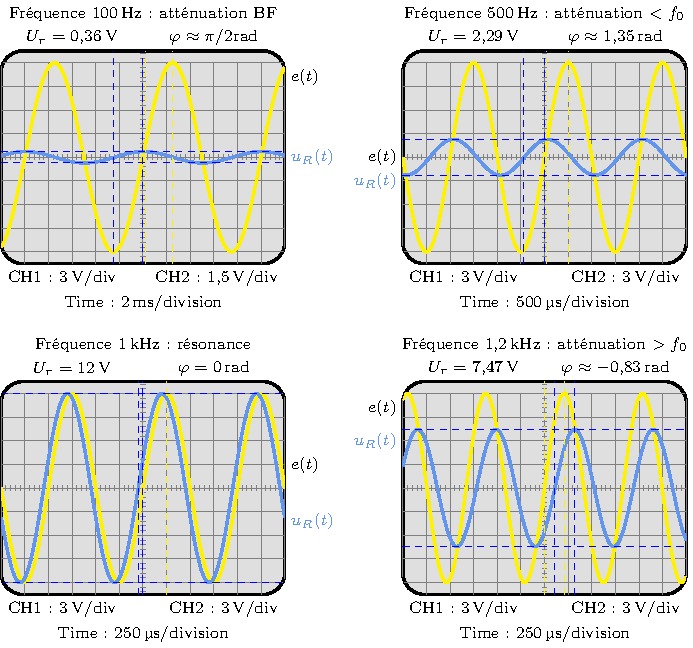
\includegraphics[width=.95\linewidth]{oscillo_intens}
\end{center}

On remarque que~:
\begin{itemize}
    \item à une fréquence \textbf{très inférieure} à la fréquence de résonance,
        par exemple \SI{100}{Hz} (un dixième de $f_0$), la tension (donc
        l'intensité) est \textbf{presque nulle} par rapport à ce qu'impose
        l'entrée. De plus, le signal de sortie est \textbf{en avance}, avec
        une phase de $\pi/2$ (en avance car son maximum arrive avant celui du
        GBF)~;
    \item à une fréquence \textbf{un peu inférieure} à $f_0$, par exemple
        \SI{500}{Hz} ($f_0/2)$, la sortie \textbf{est atténuée}, mais toujours
        \textbf{en avance}~;
    \item à la \textbf{fréquence de résonance}, l'amplitude de la tension de la
        résistance (donc l'intensité à un facteur $R$ près), est
        \textbf{maximale} et est \textbf{en phase} avec le signal d'entrée (les
        maxima arrivent au même moment)~;
    \item à une fréquence \textbf{un peu supérieure} à $f_0$, par exemple
        \SI{1200}{Hz} ($\num{1.2}f_0$), on retrouve une \textbf{atténuation},
        mais cette fois le signal est \textbf{en retard} sur l'entrée (son
        maximum arrive après celui de $e(t)$).
    \item Pour une fréquence \textbf{très supérieure} à la fréquence de
        résonance, par exemple \SI{10}{kHz} ($10f_0$), on retrouve la même
        atténuation qu'à $\num{0.1}f_0$ mais la phase est opposée.
\end{itemize}

\begin{enumerate}[label=\sqenumi, start=4]
    \item Ainsi, on relève les valeurs d'amplitude et de décalage temporel entre
        les signaux à chaque fréquence d'entrée choisie~: on obtient la phase
        avec la relation
        \[\D\f = \w\D t =2\pi f\D t\]
        étant donné que par définition, la phase est la vitesse angulaire de la
        phase ($\w = \D\f/\D t$ comme $v = d/t$). On trouve alors les courbes
        suivantes~:
\end{enumerate}
\begin{center}
    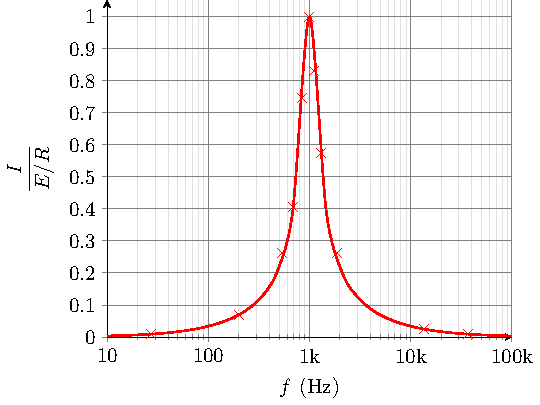
\includegraphics[width=.49\linewidth]{RLCR_amplitude}
    \hfill
    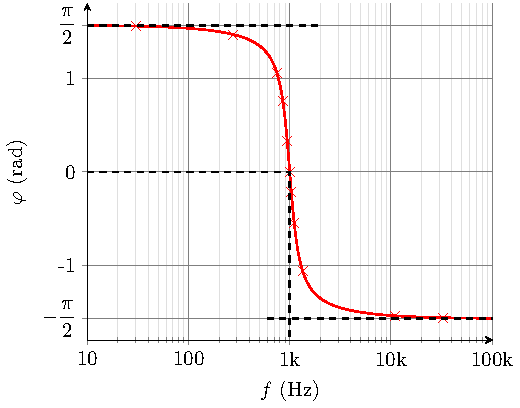
\includegraphics[width=.49\linewidth]{RLCR_phase}
\end{center}

\section{Valider et conclure}

\begin{enumerate}[label=\sqenumi, start=5]
    \item On trouve en effet que les courbes ont l'allure attendue, aux erreurs
        de mesure près compte-tenu des incertitudes de lecture et des
        incertitudes sur la valeur exacte des composants.
    \item La largeur de la bande passante, en revanche, ne correspond pas à la
        théorie~: elle est plus large que prévue~! En effet, le facteur de
        qualité du circuit $Q = 1/R\sqrt{L/C}$ prend en compte indifféremment
        toutes les résistances du circuit~: il y en a dans l'inductance (autour
        de $\SI{50}{\Omega}$), dans le condensateur, dans les câbles… et donc $Q$
        est plus petit que ce que prévoit la théorie~:
        \begin{gather*}
            R_{\rm circuit} > R\\
            \Leftrightarrow
            Q_{\text{réel}} = \frac{1}{R_{\rm circuit}} \sqrt{\frac{L}{C}}
            <
            Q_{\rm theo} = \frac{1}{R} \sqrt{\frac{L}{C}}
        \end{gather*}
            Ainsi, comme la bande passante est définie par $\D\w = \w_0/Q$, on a
            \[\boxed{\D\w_{\text{réel}} > \D\w_{\rm theo}}\]
\end{enumerate}

\end{document}
